\documentclass[12pt]{report}
\usepackage[top=23mm,bottom=23mm,left=23mm,right=23mm]{geometry}
\usepackage{fancyhdr, lastpage}
\usepackage{times}
\usepackage{chapterbib}
\usepackage[sectionbib]{natbib}
\bibpunct{(}{)}{;}{a}{,}{,}
\usepackage[pdftex]{graphicx}
\usepackage{epstopdf}
\usepackage{subfigure}
\usepackage[footnotesize, bf]{caption}
\usepackage{amsmath}
\usepackage{amssymb}
\usepackage{amsthm}
\usepackage{setspace}
\usepackage[small,compact]{titlesec}
\usepackage{multicol}
\usepackage{multirow}
\usepackage{wrapfig}
% \usepackage{minitoc}  Was not compatible with anything
\usepackage{array}
\usepackage{tikz}
\usepackage{enumerate}  % for enumerating with a), b) etc...
\usepackage{caption}    % for having enumertion in a caption 
\usepackage{cleveref}   % So multiple references will auto format themself
\usepackage{algorithm2e}
%\usepackage{hyperref}   % This allows for hyperlinks in the table of content
%\hypersetup{
%  colorlinks,
%  citecolor=black,
%  filecolor=black,
%  linkcolor=black,
%  urlcolor=black
%}

\usepackage[mathlines]{lineno}  % Line numbers in document...
\usepackage{silence}

%% parameters for lineno to work nicely
\linenumbers
\makeatletter
% Make a copy of macros responsible for entering display math mode
\let\start@align@nopar\start@align
\let\start@gather@nopar\start@gather
\let\start@multline@nopar\start@multline
% Add the "empty line" command to the macros
\long\def\start@align{\par\start@align@nopar}
\long\def\start@gather{\par\start@gather@nopar}
\long\def\start@multline{\par\start@multline@nopar}
\makeatother

%% Thereom and Proposition stuff
\theoremstyle{plain}
\newtheorem{thm}{Theorem}[section]
\newtheorem{prop}[thm]{Proposition}

%% Supress annoying warnings
\WarningFilter{latex}{Text page}

%Folder paths that contain graphics
\graphicspath{
  {./}
  {Chapters/3_numerics/figs_method_comparisons/}
  {Chapters/3_numerics/figs_method_description/}
  {Chapters/4_simulation/Figures/}
  {Chapters/4_simulation/Show1DFigures}
}

% PDF hyper-linking (set colors to black for printing)
%\usepackage[ps2pdf=true,colorlinks]{hyperref}
%\usepackage[figure,table]{hypcap}
%\hypersetup{
%	bookmarksnumbered,
%	pdfstartview={FitH},
%	citecolor={black},
%	linkcolor={black},
%	urlcolor={black},
%	pdfpagemode={UseOutlines}
%}

\pdfinfo{
/Author (Eric M. Jalbert, 2015)
/Title (Numerical Analysis of Methods for Simulating Clostridium Thermocellum)
/Subject (Numerical Analysis of Methods for Simulating Clostridium Thermocellum)
}

%Paragraph symmetries...
\setlength{\parskip}{10pt}
\setlength{\parindent}{0pt}
\setlength{\parsep}{0pt}


\setcounter{secnumdepth}{5}
\setcounter{tocdepth}{1}
%\setcounter{minilofdepth}{2}
\renewcommand{\abstractname}{\Large ABSTRACT}
\renewcommand{\bibname}{References}
%\renewcommand\bibsection{}
%\renewcommand{\bibsep}{0pt}

\setlength{\headheight}{15pt}

\fancypagestyle{custom}{
\lhead{\textit{E.Jalbert, 2014}}
\rhead{\textit{NUMERICAL ANALYSIS SIMULATING C.THERMOCELLUM}}
}

\fancypagestyle{References}{
\lhead{}
\rhead{\textit{REFERENCES}}
}

%%%%%%%%% If I have appendies, add the fancy page styles 
%%%%%%%%% like the example below
%\fancypagestyle{AppendixA}{
%\lhead{}
%\rhead{\textit{APPENDIX A: Default Simulation Parameters}}
%}

\begin{document}

%PreliminarySections
\pagenumbering{roman}
%----------------------------------------------------------
% Title Page
%   The first page of the thesis, contains 
%   author/university/title and other info
%----------------------------------------------------------
\begin{titlepage}
  \begin{center}
    \vspace*{4cm}
    \LARGE\large{Comparison of a Semi-Implicit and a Fully-Implicit Time Integration Method for a Highly Degenerate Diffusion-Reaction Equation Coupled with an Ordinary Differential Equation}
    \vspace*{0.5cm}
    
    \small{by}
    \vspace*{0.5cm}
    
    \large{Eric M. Jalbert}
    \vspace*{3.5cm}
    
    A Thesis\\presented to\\The University of Guelph
    \vspace*{1.5cm}
    
    In partial fulfilment of requirements\\for the degree of\\Master of Science\\in\\Applied Mathematics
    \vfill

    Guelph, Ontario, Canada
    
    $\copyright$ E.M. Jalbert, January, 2015
  \end{center}
\end{titlepage}






%%Abstract
%\phantomsection
\addcontentsline{toc}{section}{Abstract}
%\section*{ABSTRACT}
\begin{abstract}
\setcounter{page}{2}
\begin{center}
%\vspace*{33pt}
\large{\textbf{Comparison of a Semi-Implicit and a Fully-Implicit Time Integration Method for a Highly Degenerate Diffusion-Reactor Equation Coupled with and Ordinary Differential Equation}}\\
\vspace*{20pt}
\begin{minipage}{0.49\textwidth}
\begin{flushleft}
\normalsize{Eric M. Jalbert}\\
\normalsize{University of Guelph,2015}
\end{flushleft}
\end{minipage}
\begin{minipage}{0.49\textwidth}
\begin{flushright}
\normalsize{Advisor}\\
\normalsize{Professor Hermann J. Eberl}
\end{flushright}
\end{minipage}
\end{center}
\vspace*{20pt}

%Degenerate diffusion-reaction equations tend to arise when modelling biofilm growth and propagations.
%Specifically focusing on \textit{Clostridium thermocellum}, because of its potential in the field of energy biotechnology, the model by \cite{dumitrache2015mathematicalModeling} is extended for spatial consideration.
%The resulting system is a partial differential equation coupled with an ordinary differential equation, these correspond to the diffusing biomass and the non-diffusing substrate.
%This introduces a degeneracy at the interface which makes typical numerical computations of the solution difficult.
%For this, a fully-implicit time integration method is formulated so that it generalises a semi-implicit method to solve the problem with addition accuracy.
%The fully-implicit method uses a fixed-point iteration and preselected tolerance to approximate the solutions at the next time step.
A certain class of highly degenerate diffusion equations arises when modelling biofilm growth and propagations.
We focus on the cellulolytic \textit{Clostridium thermocellum}, because of its potential in the field of energy biotechnology.
From this system a spatially implicit model was proposed in the literature before.
Here we study a spatially explicit model.
In contrast to other biofilm systems, a special feature of this system is that the growth promoting nutrient is not diffusive but bound in the substratum on which the biofilm grows.
As a consequence one obtains a highly degenerate diffusion-reaction equation for the bacteria that is coupled to an ordinary differential equation for nutrients.
The degeneracy of the biomass equation introduces gradient blow-up at the interface which makes numerical treatment difficult.
For this, a fully-implicit time integration method is formulated so that it generalises a previously used semi-implicit method to solve the problem with increased accuracy.
The fully-implicit method uses, at each time-step, a fixed-point iteration to solve the arising nonlinear algebraic equation and can be controlled by the required tolerance for convergence.

%The newly developed method is validated and tested to investigate numerous issues that arise with numerical computations: sinks or sources of biomass, loss of characteristics in the solution, and destruction of the conservation of mass.
%Once the certainty of the solutions for the fully-implicit method are confirmed, the difference between the fully-implicit and semi-implicit methods is quantified by use of quantitative measurements so that the benefits of the new method can be recorded.
%These measurement are called the normed differences, they are the $L_1$-norm and $L_2$-norm of the relative difference between the solutions. 
%The trade-off between improved accuracy and increased computational effort is determined to be optimal for tolerances that force a single extra iteration of the fully-implicit method.
This method is validated and tested to investigate numerous issues that arise with numerical computations: mass conservations, preservation of symmetries in the initial data, and convergence with respect to grid refinement.
Furthermore, a difference is quantified between the fully-implicit and the simpler semi-implicit methods which it generalises.
The trade-off between improved accuracy and increased computational effort is found to be optimal for tolerances that force a single extra iteration of the fully-implicit method.

%The numerical method is then used to simulation the behaviour of \textit{C.thermocellum} biofilm formation on cellulose sheets with the main objective of understanding how including the spatial diffusion terms in the biomass affect the results of the simulations at a reactor-scale.
%To this end, the normal behaviour of the system was observed and compared to the results achieved by \cite{dumitrache2015mathematicalModeling}.
%Observing the typical results of the system suggested the existence of a travelling wave solution.
%While it could not be proven analytically, the existence of a travelling wave solution is strongly implied.
%To test the effect of the spatial diffusion terms, two extremes of initial biomass distributions were simulated to show that there is a quantitative difference between the behaviour but not a qualitative.
%Showing that if the spatial effects are important then a two dimensional model that includes the spatial diffusion must be used instead of a reactor-scale model that consolidated the spatial effects with a carrying capacity on the growth term.
The numerical method is then used to simulate \textit{C.thermocellum} biofilm formation on cellulose sheets with the main objectives of (i) understanding patterns of biofilm formation and (ii) understanding how including the spatial diffusion terms in the biomass affect the results of the simulations at a reactor-scale.
Our simulation results strongly suggest the formation of travelling wave solutions that describe how the biofilm moves across the substratum.
To test the effect of the spatial effects on overall biofilm performance, two extremes of initial biomass distributions were simulated.
A quantitative difference between the behaviour in both cases is found, but not a qualitative one.
This suggests that in applications where spatial heterogeneity is important then a two dimensional spatially explicit model that includes the spatial diffusion must be used instead of the earlier, simple spatially implicit reactor-scale ordinary differential equation model that consolidated the spatial effects with a carrying capacity on the growth term.
\end{abstract}


\setcounter{page}{3}
%\input{Prelims/Dedication}
%\input{Prelims/Acknowledgements}
%%\dominitoc
\setlength{\parskip}{0ex plus 0.5ex minus 0.2ex}

\tableofcontents
\pagebreak
\listoffigures
\listoftables
\setlength{\parskip}{10pt}


%%%Main Texts
\pagebreak
\pagestyle{fancy}
\pagenumbering{arabic}
\doublespacing
%\onehalfspacing

%\chapter{Introductions}
%\section{Biology Background}

This will be three to four paragraphs about the biology of this problem. That is use lots of references on biofilms and, more specifically, Clostridium Thermocellum to get some basic information down.

%\section{Objectives}

There are three main objectives of this thesis:
\begin{enumerate}
  \item Formulate and test a fully-implicit method for a highly degenerate, highly nonlinear coupled PDE-ODE system modelling \textit{C.thermocellum} biofilms. 
  \item Compare the fully-implicit method of Objective 1 with a previously introduced semi-implicit method, which it generalizes.
    This is done based on the trade-off between improved accuracy of the method and increased computational effort.
  \item Use the numerical methods developed in Object 1 and 2 to simulate \textit{C.thermocellum} biofilm formation on cellulose sheets, with the goal of understanding better the spatio-temporal dynamics of this system biofilms. 
\end{enumerate}


%\section{Thesis Outline}

\begin{itemize}
  \item Background (1.1): Describes the placement of this problem in the existing literature.
  \item Objectives (1.2): Describes the three main objectives of this thesis.
  \item Outline (1.3): Outlines the sequencial format of the thesis.
  \item Model Description (2.1): Formulates the mathematical model that is used for the rest of the study.
  \item Nondimensionalization (2.2): The system described in the previous section is reduced to unitless parameters and variables for simplicity.
  \item Discretization (3.1): Spatial and temporal discritzations are applied to the system.
  \item Solving Technique (3.2): Using a fixed-point iteration, solutions for the system are found by use of finite difference method with the Bi-Conjugate Gradiant Method and the quadratic equation.
  \item Computational Setup (3.3): The work stations and compiler settings are recorded.
  \item Method Validation (3.4): Multiple test are run to check if the handling of the spatial discritization generated any sources or sinks in the solution. A measure to compare two the solution of two different simulations is esstablished so that a grid convergence analysis can be done.
  \item Comparison of Semi-Implicit and Fully-Implicit Methods (3.5): Using the previously established measure, the semi-implicit method and fully-implicit method are compared against varying quantities and at different tolerances.
  \item Typical Simulation (4.1): A generic simulation is run to reveal the general behaviour of the system.
  \item Travelling Wave Analysis (4.2): A travelling wave solution is suggested to exist, this is tested against different simulations to reinforce the idea.
  \item Spatial Effects (4.3): The effect of ignoring the spatial diffusion is investigated by comparing two vastly different simulations; one with evenly distributed initial condition, the other with clumped initial condition.
  \item Lessons Learned (5.1): The general findings of each section are summerized.
  \item Future Work (5.2): Possible changes and extensions are discussed.
\end{itemize}


\chapter{Model}
\section{History}

%!% Try to poise the problem as an investigation of whether semi-implicit vs. fully-implicit comparison exists and assuming the fully-iomplici method is more accurate, if we actually gain anything from the extra computations

The tradition biofilm model has been continually developed over many iterations since 1980.
\cite{rittmann1980model} formulated the steady-state biofilm model, developed using the concept that biofilm growth would be the result of a steady flux from substrate.
Since then the model have evolved to include modelling three-dimensional growth of multispecies anaerobic biofilms (\cite{noguera1999simulation}) and spatially heterogeneous biofilm structures (\cite{eberl2001deterministic}). 

The modelling of \textit{Clostridium Thermocellum} is unique because this celluloytic anaerobic bacteria does not generate an extracellular polymeric substance.
This uncharacteristic behaviour means that the mathematical model based on the work of \cite{eberl2007finite} cannot be used as is. 
They modelled the biomass density and nutrient concentrations as a two-PDE-coupled system.
Recently, \cite{wang2011spatial}, used a cellular automata based model for simulating the growth of \textit{Clostridium Thermocellum}. From this, better results were thought to derive from a continuous differential equation based model.
Here the spatial diffusion of the substrait concentration is removed to mimic the carbon substrait that is consumed by \textit{Clostridium Thermocellum}. This results in a PDE-ODE-coupled system.
This is based on the work done by \cite{dumitrache2014understanding}, where this same coupling was used and formulated.

\section{Model Description}
The model used for simulations is based on the deterministic biofilm model developed in \cite{eberl2001deterministic}, which was designed for modelling the development of spatially heterogenous biofilm structures.
Since \textit{C.thermocellum} grows as a monolayered biofilm and consumes a solid carbon fibrous substrate, there are mechanical differences between the two systems.
Our model is based on the following assumptions:
\begin{enumerate}
  \item The growth of sessile biomass is limited locally by the availability of nutrients and by the availability of colonizable space.
    \label{assump:growth_inhib}
  \item The number of cells per unit area of substratum is limited to a finite value because \textit{C.thermocellum} forms only a thin monolayer. 
    \label{assump:finite_density}
  \item Biomass does not spread until its density approaches the physical limit.
    Near the physical limit it expands spatially into neighbouring regions.
    Because of this, the physical limit of biomass density is never attained.
    \label{assump:diffusion}
  \item The carbon fibrous substrate consumed as nutrition for biomass growth is the substratum to which the biofilm attaches.
    Carbon is bound in the fibers of the substratum and does not diffuse.
    The propagation of biofilm is based on the lack of available substrate locally, not the physical degradation of the substratum.
    \label{assump:substratum}
  \item Cell death and cell loss into the aqueous environment is assumed to be proportional to cell density.
    \label{assump:bio_death}
  \item Biomass growth is proportional to substrate consumption.
    \label{assump:sub_consumption}
\end{enumerate}

Assumption \ref{assump:growth_inhib}, \ref{assump:finite_density}, \ref{assump:diffusion}, \ref{assump:bio_death}, and \ref{assump:sub_consumption} are similar to those made in \cite{eberl2001deterministic}.
The main difference here is \ref{assump:substratum}; our substrate is sessile.
With a sessile substrate, there is no diffusion for the substrate concentration.
Another difference is that \textit{C. thermocellum} does not grow from the substratum into the aqueous phase.
Instead our biofilm grows across the substratum making this a two dimensional setting.

The model is formulated in a spatial domain $\Omega \subset \mathbb{R}^2$.
The independent variables $t > 0$ denote time and $x \in \Omega$ denotes the location within the physical domain.
The dependent variables are the local fraction of the surface occupied by biomass $M(t,x)$ and the substrate density $C(t,x)$.
The net growth rate of biomass is denoted by $f(C)$ and the substrate consumption rate is denoted by $g(C)$, both are dependent upon available substrate.
The diffusion coefficient that describes spatial expansion of biomass is given by the function $d(M)$.

From the above assumptions, a PDE-ODE-coupled system that models \textit{C. thermocellum} growth on carbonous fibres can be formulated as,
\begin{align} 
   M_t &= \nabla_x \left( d(M) \nabla_x M \right) + f(C) M \label{equ:model_M}\\
   C_t &= -g(C) M \label{equ:model_C}
\end{align}
where
\begin{equation} \label{equ:model_d}
  d(M) = d \frac{M^\alpha}{(1-M)^\beta}
\end{equation}
\begin{equation} \label{equ:model_f}
  f(C) = u \frac{C}{k_C + C} - n 
\end{equation}
\begin{equation} \label{equ:model_g}
  g(C) = y \frac{C}{k_C + C}
\end{equation}
with all parameters non-negative.
Here we have a pair of equations, (\ref{equ:model_M}) and (\ref{equ:model_C}), that represent the biomass density and substrate concentration respectively.
This is a model for spatially explicit biomass growth.
This agrees with assumption \ref{assump:diffusion} since for $0 < M \ll 1$ the spreading effect is negligible but when $0 \ll M \approx 1$ there is considerable spreading.
This choice for a spatially considerate model is based on the work done in \cite{khassehkhan2009nonlinearMaster}.
By assumption \ref{assump:growth_inhib}, the only factors affecting the biomass density is growth from nutrient conversion and diffusion from local spatially-full colonized space.
For equation (\ref{equ:model_d}), the density-dependent diffusion equation, $d$ is the diffusion coefficient which controls the magnitude of the diffusion and the parameters $\alpha$ and $\beta$ are selected to control the strength of the diffusion.
For equation (\ref{equ:model_d}) the diffusion term is shown to have the wanted behaviour since it has a near-zero finite value until $M \to 1$, which leads to $d(M) \to \infty$ as seen in Figure \ref{fig:show_d}. 
The production rate is the difference between simple Monod kinetic growth term, with growth rate $u$, and a constant death rate term, $n$, to agree with assumption \ref{assump:growth_inhib} and \ref{assump:bio_death}.
Monod kinetic growth was selected, with half-saturation carbon concentration $k_C$, since it matches the growth of bacteria when limited by available nutrients. %!% citation here?

Equation (\ref{equ:model_C}) describes the consumption of carbon substrate due to biomass growth.
Parameter $y$ is the consumption rate, measured in mass carbon per unit time.
Substrate consumption is proportional to the local biomass density $M$. 
Parameter $k_C$, same as in the growth term for (\ref{equ:model_M}), is again the half-saturation carbon concentration.
Here assumption \ref{assump:substratum} and \ref{assump:sub_consumption} are satisfied since there exists no diffusion term for the substrate and its growth is a scalar multiple of the biomass growth rate.


\begin{figure}
  \centering
  \begin{tikzpicture}[scale = 4]
    \draw[<->, thick] (1.1,0) -- (0,0) -- (0,1);
    \draw[dashed] (0.95,0) -- (0.95,1.4);

    \node[below] at (0.95,0) {$1$};
    \draw (0.95, 0.02) -- (0.95, -0.02);

    \node[right] at (1.1,0) {$M$};
    \node[above] at (0,1.1) {$d(M)$};

    \draw[->, domain=0:0.92, samples=100] plot (\x, {0.0001*pow(\x/(1-\x+0.01), 4)});
  \end{tikzpicture}
  \caption{A graph of $d(M) = d \frac{M^\alpha}{(1 - M)^\beta}$ showing the way diffusion increases asymptotically as $M \to 1$.}
  \label{fig:show_d}
\end{figure}

%!% l.307-311 this paragraph seems somewhat out of place here
It has been shown in \cite{jalbert2014numerical} that for the solutions of these kinds of degenerate problems a finite speed of interface propagation exists, where $d(0) = 0$ and $\alpha >1$ in (\ref{equ:model_d}).
These problems have a blow up in the biomass gradient at the interface because of the degeneracy that exists there.
%!% HERB: This property should be stated as a theorem and proved.
For this system, we have $M < 1$ always since the diffusion when $M \approx 1$ is great enough to always ensure this \citep{jalbert2014numerical}.

 
The dimensions of the parameters and variables are in Table \ref{tab:varDimensions}.
Note that since we have a two dimensional problem, due to the lack of complex biofilm structures from \textit{C. thermocellum} growth, the spatial considerations are all strictly for area and not volume, as is typically done for biofilm modelling.
  \begin{table}[!hbt]
    \centering
    \begin{tabular}{|l |c |l |}
      \hline 
      Description & Symbol & Dimensions \\
      \hline
      \hline
      Spatial region & $\Omega$ &  $NA$ \\
      \hline 
      Time & $t$ & $\left[days\right]$ \\
      Location in $\Omega$ & $x=(x_1,x_2)$ & $\left[meters, meters\right]$ \\
      \hline
      Biomass fraction & $M$ & $\left[-\right]$ \\
      Substrate concentration & $C$ & $\left[\frac{grams}{meters^2}\right]$ \\
      \hline
      %!% Should this be meters^2 or meters?, I think it doesn't work unless it is meters^2 but I had Meters
      Diffusion coefficient & $d$ & $\left[\frac{meters^2}{days}\right]$ \\
      Density-dependent exponent & $ \alpha $ & $\left[-\right]$  \\
      Density-dependent exponent & $ \beta  $ & $\left[-\right]$  \\
      Growth rate & $ u $ & $\left[days^{-1} \right]$ \\
      Half-saturation carbon concentration & $ k_C $ & $\left[\frac{grams}{meters^2}\right]$ \\
      Maximum consumption rate & $y$ & $\left[\frac{grams\ carbon}{days}\right]$  \\
      Death constant & $n$& $\left[days^{-1} \right]$ \\
      \hline
    \end{tabular}
    \caption{List of parameters and their dimensions}
        \label{tab:varDimensions}
  \end{table}

The model (\ref{equ:model_M}), (\ref{equ:model_C}) is completed by boundary conditions for the biomass density, $M$, and initial conditions for both $M$ and substrate concentration $C$.
For $M$ we pose homogeneous Neumann boundary conditions such that,
\begin{equation} 
  \partial_n M = 0, \quad x \in \partial \Omega.
\end{equation}
The initial conditions for the biomass density is,
\begin{equation}
  M(0,x) = M_0(x), \quad x \in \Omega,
\end{equation}
where $0 \le M_0(x) < 1$ and $M_0(x)$ non-zero in specific pockets on the substratum. 
These are specified below for each individual, simulation experiments.
The initial conditions for the substrate concentration is,
\begin{equation}
  C(0,x) = C_{\infty}, \quad x \in \Omega,
\end{equation}
where $C_{\infty}$ describes the initial carbon density in the substratum.


\section{Nondimensionalization}
 

To help facilitate the analysis of this system, the full removal of all physical units is preferred and so we nondimensionalize the parameters.
Here the parameters used are: the biomass growth rate, $u$; the length of the region, $L$; and the maximum density for biomass and substrate, $M_\infty$ and $C_\infty$.
The biomass density fraction represents the current density of biomass divided by the maximum biomass density, $M_{\infty}$.
From using the following parameter changes, the system can be made unitless.
\begin{align}
  \chi &= \frac{x}{L} \implies L d\chi= dx \\
  \tau &= u t \implies \frac{1}{u} d\tau= dt \\
  \mathcal{C} &= \frac{C}{C_{\infty}} \\
  \delta &= \frac{1}{u L^2} d \\
  \kappa &= \frac{k}{C_\infty} \\
  \nu &= \frac{n}{u C_\infty} \\
  \gamma &= \frac{M_\infty}{C_\infty} y
\end{align}

%%%%%%%% This section seems a little too pedantic for a thesis, Also it needs notations change and probably has errors....
% This gives the system
% \begin{align}
%   \mathcal{M}_\tau &= \frac{1}{u L^2} \nabla_\chi \left(D(m) \nabla_\chi M \right) + \frac{1}{u} F(\mathcal{C}) \mathcal{M} \\ 
%   \mathcal{C}_\tau &= \frac{ -1}{\mathcal{C}_\infty u} G(\mathcal{C}) \mathcal{M}
% \end{align}
% 
% where 
% \begin{equation}
%   D(M) = {u L^2 \delta} \frac{M^\alpha}{(1-M)^\beta}
% \end{equation}
% 
% \begin{equation}
%   F({\mathcal{C}}) = \frac{{u} {\mathcal{C} \mathcal{C}_0}}{{\kappa \mathcal{C}_0} + {\mathcal{C} \mathcal{C}_0}} M \left(1 - \left( \frac{M}{{\mathcal{C}}} \frac{M_0}{\mathcal{C}_0} \right)^\gamma \right) \\
% \end{equation}
% 
% \begin{equation}
%   G({\mathcal{C}}) = -\frac{{u \mathcal{C}_0 \nu} {\mathcal{C} \mathcal{C}_0}}{{\kappa \mathcal{C}_0} + {\mathcal{C} \mathcal{C}_0}} M \\
% \end{equation}
% 
% This can be greatly simplified by cancelling out parameters.
% 
% \begin{align}
%   M_\tau &= \nabla_\chi \left( {\delta} \frac{M^\alpha}{(1-M)^\beta} \nabla_\chi M\right) + \frac{ \mathcal{C} }{{\kappa } + {\mathcal{C}}} M \left(1 - \left( \frac{M}{{\mathcal{C}}} \frac{M_0}{\mathcal{C}_0} \right)^\gamma \right) \\
%   \mathcal{C}_\tau &= - \frac{\nu \mathcal{C}}{\kappa + \mathcal{C}} M
% \end{align}
% 
% Now we can name functions and get the final nondimensionalized system.

Using these, (\ref{equ:model_M}) and (\ref{equ:model_C}) can be simplified and nondimensionalized into, 
\begin{align} \label{equ:model_system}
  M_\tau &= \nabla_\chi \left( D(M) \nabla_\chi M \right) + F(\mathcal{C}) M \\
  \mathcal{C}_\tau &= - G(\mathcal{C}) M, 
\end{align}

where,

\begin{equation}
\begin{aligned} \label{equ:model_functions}
  D(M) &= \delta \frac{M^\alpha}{(1 - M)^\beta} \\
  F(\mathcal{C}) &= \frac{ \mathcal{C}} {\kappa + \mathcal{C}} - \nu \\
  G(\mathcal{C}) &= \gamma \frac{\mathcal{C}}{\kappa +\mathcal{C}}.
\end{aligned}
\end{equation}
with only $\delta, \kappa, \nu, \gamma$ as model parameters. 
For convience, we henceforth use
\begin{equation}
  C := \mathcal{C},\quad x := \chi,\quad t := \tau.
\end{equation}

Each of the dimensionless parameters in (\ref{equ:model_functions}) have a biological representation based on the transformations done.
The parameter $\delta$ is the dimensionaless biomass motility coefficient.
It affects the change in biomass from adjacent biomass sources, a greater $\delta$ results in faster biofilm expansion.
The parameter $\kappa$ is the half-saturation point, it is exactly the value for which substrate concentration results in $0.5$-optimum growth rate.
Parameter $\nu$ is the decay and loss rate for biomass.
These can be from starvation in cases where substrates are depleted or from loss into the aqueous enviroment.
Lastly, $\gamma$ is the dimensionless maximum substrate consumption rate.
It signifies the ratio of substrate consumed to biomass growth.
Here, a larger $\gamma$ value results in more substrate being consumed to  produce the same amount of biomass. 

With (\ref{equ:model_system}) being reduced to these parameters the numerical analysis become more simiplified while still retaining the same significance in results.

\section{Parameters}

Each of the dimensionless parameters in (\ref{equ:model_functions}) have a biological representation based on the transformations done.
The parameter $\delta$ is the dimensionaless constant for diffusion.
It affects the change in biomass from adjacent biomass sources, a greater $\delta$ results in a greater change.
The parameter $\kappa$ is the half-saturation point, it is exactly the value for which substrait concentration results in $0.5$-optimum growth rate.
Parameter $\nu$ is the death rate of the biomass.
Specifically, it is the ratio of biomass growth to death, representing the fraction of biomass density that perishs from natural causes or a lack of substrait.
Lastly, $\gamma$ is the yield ratio.
It signifies the ratio of substrait consumed to biomass growth.
Here, a larger $\gamma$ value results in more substrait being consumed to  produce the same amount of biomass. 

With (\ref{equ:model_system}) being reduced to four parameters the numerical analysis become more simiplified while still retaining the same significance in results.

\chapter{Numerics}
\section{Discritization}

In order to find the solution for (\ref{equ:model_system}) spatial and temporal discritizations must be made.
First the equations are discritzied by time, 
\begin{equation} \label{equ:M_time_discrit}
  \frac{M^{k+1} - M^{k}}{\Delta t} = \nabla_x (D(M^{k+1}) \nabla_x M^{k+1}) + F(C^{k+1}) M^{k+1},
\end{equation}
\begin{equation} \label{equ:C_time_discrit}
  \frac{C^{k+1} - C^{k}}{\Delta t} = \frac{h}{2} ( G(C^{k+1}) M^{k+1} + G(C^{k}) M^{k} ).
\end{equation}
Here, (\ref{equ:M_time_discrit}) follows the ideas of the Backwards Euler Method; (\ref{equ:C_time_discrit}) follows Trapezoidal Rule. 
The index variable $k$ has also been introduced in (\ref{equ:M_time_discrit} - \ref{equ:C_time_discrit}) as time step counting variable.

Now, only (\ref{equ:M_time_discrit}) requires spatial considerations since, according to the biology of our system, the substrate does not diffuse across the region.
The spatial discritization will be through the Finite Difference Method as described in \cite{saad2003iterativeMethod}.
Here a grid will be created over the region and the solution of (\ref{equ:M_time_discrit}) will be approximated at each grid point using a five-point stencil. 
This results in, 
\begin{equation} \label{equ:M_space_discrit}
  \frac{M^{k+1}_{i,j} - M^{k}_{i,j}}{\Delta t} = 
    \frac{1}{\Delta x^2} \sum_{(s,r) \in \mathbb{A}} \left( D(M^{k}_{i+\frac{s}{2}, j+\frac{r}{2}}) \cdot
    ( M^{k+1}_{i+s, j+r} - M^{k+1}_{i,j}) \right) + F(C^{k}_{i,j}) M^{k+1}_{i,j}
\end{equation}
where $\mathbb{A} = \left\{ (0, \pm1), (\pm1, 0) \right\}$.
Now there are two additional indexing variables, $i$ and $j$.
These count out the respective grid point for the spatial discritization.
On a $n \times m$ grid, the $x_1$ and $x_2$ dimensions would be represented by $i \in (0, n)$ and $j \in (0,m)$ respectivly.
One item to note is that the index on $D$ is halved because it is the arithmetic average of two adjacent values.

Now (\ref{equ:C_time_discrit}) and (\ref{equ:M_space_discrit}) can be solved as a fixed-point-iteration method.
In a single time step, the solutions for $M$ and $C$ can be solved using the previous time step solution in the follow manner:
\begin{equation} \label{equ:M_fixed_point}
  \frac{M^{p+1}_{i,j} - M^{k}_{i,j}}{\Delta t} = 
    \frac{1}{\Delta x^2} \sum_{(s,r) \in \mathbb{A}} \left( D(M^{p}_{i+\frac{s}{2}, j+\frac{r}{2}}) \cdot
    ( M^{p+1}_{i+s, j+r} - M^{p+1}_{i,j}) \right) + F(C^{p}_{i,j}) M^{p+1}_{i,j}
\end{equation}
\begin{equation} \label{equ:C_fixed_point}
  \frac{C^{p+1} - C^{k}}{\Delta t} = \frac{-1}{2} ( G(C^{p+1}) M^{p+1} + G(C^{k}) M^{k} )
\end{equation}
where $p \in (0,P)$, and for $p = 0$ we have $M^0 = M^{k}, C^0 = C^{k}$, and for $p = P$ we have $M^{P} = M^{k+1}, and C^{P} = C^{k+1}$.



\section{Solution Technique}

%!% ...a coupled system of $2nm$ highly... | Makes sure 2nm is the correct amount of points based on \pi, Hermann suspects 2(n+1)(m+1)
Assuming the values for $C$ and $M$ at time level $k$ are known, (\ref{equ:M_space_discret}) and (\ref{equ:C_space_discret}) are a coupled system of $2nm$ highly nonlinear equation for $2nm$ unknown $M^{k+1}_{l}$, $C^{k+1}_{l}$.
To solve this coupled system, we define a fixed point iteration which we apply to (\ref{equ:M_space_discret}) and (\ref{equ:C_space_discret}).
In a single time step, the solutions for $M$ and $C$ can be solved using the previous time step solution in the follow manner:
%!% HERB, describe how the selection of (p), (p+1), and k are made such that it is very clear
\begin{equation} \label{equ:M_fixed_point}
  \frac{M^{(p+1)}_{l} - M^{k}_{l}}{\Delta t} = 
    \frac{1}{\Delta x^2} \sum_{\sigma \in \mathcal{N}_{\pi^{-1}(l)}}
    \left( \frac{D(M^{(p)}_{\pi(\sigma)}) + D(M^{(p)}_{l})}{2} \right)
    \cdot \left( M^{(p+1)}_{\pi(\sigma)} - M^{(p+1)}_{l} \right)
    + F(C^{(p)}_{l}) M^{(p+1)}_{l}
\end{equation}
\begin{equation} \label{equ:C_fixed_point}
  \frac{C^{(p+1)}_{l} - C^{k}_{l}}{\Delta t} = \frac{1}{2} ( G(C^{(p+1)}_{l} ) M^{(p+1)}_{l} + G(C^{k}_{l}) M^{k}_{l} )
\end{equation}
where $(p) \in (0,1,2,\ldots)$, $(p+1)$ is the next iteration solution fo $p$, and $k$ is the solution of the previous timestep.
An initial guess is made such that,
\begin{equation}
  M^{(p)}_{l} := M^{k}_{l}, \quad C^{(p)}_{l} := C^{k}_{l}.
\end{equation}
The fixed-point iteration is stopped when convergence is achieved.
This is when the difference between consecutive iterations is below a selected tolerance, i.e.
\begin{equation} \label{equ:iteration_convergence}
  %!% The upper sum index might not be nm, maybe (n+1)(m+1)-1
  \sum^{nm}_{l=1} \left( \left| M^{(p+1)}_{l} - M^{(p)}_{l}\right| + \left| C^{(p+1)}_{l} - C^{(p)}_{l} \right| \right) < tol.
  %!% HERB, check if M^(p+1) = M^(p) and same for C for all x, such that from iteration p to p+1 we stayed fixed at the same point, is it clear that equations (3.11) - (3.12) are satisfied by these two functions? ie that they are at a fixed point, I ask because you don't just write iteration you always write "fixed-point" iteration.
\end{equation}
At the end of the fixed-point iteration, the number of iterations is recorded as $P$, and we define,
\begin{equation}
  M^{k+1}_{l} := M^{(P)}_{l}, \quad C^{k+1}_{l} := C^{(P)}_{l}.
\end{equation}
In this fixed point format, given by (\ref{equ:M_fixed_point}) - (\ref{equ:C_fixed_point}), the equations can be rearranged and solved by conventional methods.

In each iteration step, (\ref{equ:M_fixed_point}) is a simultaneous linear system for the $nm$ unknown $M^{(p+1)}_{l}$.
From this a linear system of equations can be created following \cite{saad2003iterativeMethod}.
%!% This is not needed since this information is already in equ:M_fixed_point
%For each grid point, $l$ a linear system is defined as:
%\begin{equation} \label{equ:M_linear_equation}
%\begin{aligned}
%  \frac{1}{\Delta t}M^{k}_{l} &=
%  -\sum_{\sigma \in \mathcal{N}_{\pi^{-1}(l)}} \left( \frac{D(M^{(p)}_{\pi(\sigma)}) + D(M^{(p)}_{l})} 
%    {2\Delta x^2} \cdot M^{(p+1)}_{\pi(\sigma)} \right) \\
%  & +\sum_{\sigma \in \mathcal{N}_{\pi^{-1}(l)}} \left( \left( \frac{ D(M^{(p)}_{\pi(\sigma)}) + D(M^{(p)}_{l})} 
%    {2\Delta x^2} \right) - F(C^{(p)}_{l}) + \frac{1}{\Delta t} \right) M^{(p+1)}_{l}.
%\end{aligned}
%\end{equation} 

%!% OLD From (\ref{equ:M_linear_equation}), we get the matrix equation:
From (\ref{equ:M_fixed_point}), we get the matrix equation:
\begin{equation}
  A^{(p)}M^{(p+1)} = \frac{1}{\Delta t} M^{k}.
\end{equation}
Here, $A^{(p)}$ is a five-diagonal $nm \times nm$ matrix, defined as
%!% l.408 the range of your matrix entries is off and needs to be fixed.
\begin{equation} \label{equ:M_matrix_form}
  A^{(p)} = 
  \begin{tikzpicture}[baseline=(current bounding box.center)]
    \matrix (m) [matrix of math nodes, style={nodes={rectangle,minimum width=4em}}, nodes in empty cells, right delimiter={]}, left delimiter={[}]
    {
    a_{1,1} & a_{1,2} & & a_{1,m} & & & & \\
    a_{2,1} & & & & & & & \\
    & & & & & & & \\
    a_{n,1} & & & & & & & \\
    & & & & & & & a_{nm-n, nm} \\
    & & & & & & & \\
    & & & & & & & a_{nm-1, nm} \\
    & & & & a_{nm,nm-m} & &  a_{nm,nm-1} & a_{nm,nm} \\
    } ;
    \draw[thick, loosely dotted] (m-1-1) -- (m-8-8);
    \draw[thick, loosely dotted] (m-1-2) -- (m-7-8);
    \draw[thick, loosely dotted] (m-2-1) -- (m-8-7);
    \draw[thick, loosely dotted] (m-4-1) -- (m-8-5);
    \draw[thick, loosely dotted] (m-1-4) -- (m-5-8);
  \end{tikzpicture}
\end{equation}
where each $a_{i,j}$ is the coefficient for specific grid indices based on (\ref{equ:M_fixed_point}). %OLD (\ref{equ:M_linear_equation}).

\begin{prop} \label{prop:pos_sym}
 If $ \Delta t < \left( { F(C^{(p)}_{l}) } \right)^{-1}$ then the matrix $A$ is positive definite and symmetric.
\end{prop}
\begin{proof}
  Matrix $A$ is positive definite if all the eigenvalues are positive. 
%!% l.413 to make this line of argumentation cleare it would be good to point out that the diagonal elements of the matrix are all positive. Gershgorin's theorem is not a theorem on positivity of eigenvalues, but it says that the eigenv:alues are conatained in the gershgorin discs around the diagonal elements. That beeing said, you need positive diagonals to make this work.
  Using the Gershgorin's Circle theorem described by \cite{varga2004gersgorin}, the eigenvalues can be shown to be positive.
  Gershgorin's Circle theorem tells us that each eigenvalue must be contained in the union of all Gershgorin's discs \citep{varga2004gersgorin}.
  There exist one disc for each row of $A$, with radius equal to the sum of the off-diagonals and center equal to the value of the main diagonal.
  By showing that, independently on all rows, the sum of the off-diagonals values is less then the diagonal value we have that all the Gershgorin's discs must be in the positive region when the main diagonal is positive.
  This can be shown by manipulating (\ref{equ:M_fixed_point}) for just the main diagonal element,
  \begin{equation} \label{equ:main_diagonal}
    \sum_{\sigma \in \mathcal{N}_{\pi^{-1}(l)}} \left( 
      \left( \frac{D(M_{\pi(\sigma)}^{(p)}) + D(M_l^{(p)})}{2\Delta x^2} \right)
      - F(C_l^{(p)}) + \frac{1}{\Delta t} \right) M_l^{(p+1)}
  \end{equation}
  and for just the off-diagonal elements,
  \begin{equation} \label{equ:off_diagonal}
    \sum_{\sigma \in \mathcal{N}_{\pi^{-1}(l)}} \left( 
      \left( \frac{D(M_{\pi(\sigma)}^{(p)}) + D(M_l^{(p)})}{2\Delta x^2} \right)
      M_{\pi(\sigma)}^{(p+1)} \right).
  \end{equation}
  Comparing the coefficients to the vector elements in (\ref{equ:main_diagonal}) - (\ref{equ:off_diagonal}) results in the inequality nesseccary for Gershgorin's Circle theorem.
  \begin{equation} \label{equ:diagonalGreatOffdiagonal}
    \left| \sum_{\sigma \in \mathcal{N}_{\pi^{-1}(l)}} 
      \frac{D(M_{\pi(\sigma)}^{(p)}) + D(M_l^{(p)})}{2\Delta x^2} 
      \right| 
    <
    \left| \sum_{\sigma \in \mathcal{N}_{\pi^{-1}(l)}} \left( 
      \frac{D(M_{\pi(\sigma)}^{(p)}) + D(M_l^{(p)})}{2\Delta x^2} \right)
      - F(C_l^{(p)}) + \frac{1}{\Delta t} \right|
  \end{equation}
  This simplifies to,
  \begin{equation} \label{equ:proof_inequality}
    \Delta t < \left( { F(C^{(p)}_{l}) } \right)^{-1} 
  \end{equation}
  When this inequality is true, we have that the off-diagonals are smaller then the main diagonal and the main diagonal values are positive thus Gershgorin's Circle theorem says that the eigenvalues are all positive.
  Therefore we have positive definite when (\ref{equ:proof_inequality}) is true.

  The symmetry of $A$ can be trivially shown if one considers the formation of the diagonals.
  On a single row, each element corresponds to the adjacent grid points of grid $l$.
  As the grid ordering counts along, the elements that are equi-distance from the diagonal actually reference the same grid point. 
  Therefore we have symmetry. 
\end{proof} 

It is important to remark that the time-step constraint in Proposition \ref{prop:pos_sym} is not a severe constraint, practically.
The condition, $\frac{1}{F(C)} < \Delta t$, relates the growth of the biomass to the size of time step selected.
In order to resolve any biomass growth, $\Delta t$ must obviously be chosen smaller then the characteristic time scale of growth ,$\frac{1}{F(C)}$.

Given that $A$ is positive definite and symmetric, the conjugate gradient method can be used to compute the solution.

\begin{prop}
  The matrix $A$ is diagonally dominant when $\Delta t < \left( { F(C^{(p)}_{l}} \right)^{-1}$.
\end{prop}
\begin{proof}
  This is trivially shown to be true when one considers (\ref{equ:diagonalGreatOffdiagonal}).
  It was shown that this simplifies to 
  \begin{equation}
    \Delta t < \left( { F(C^{(p)}_{l}) } \right)^{-1}
  \end{equation}
  This means that when the above is true the diagonal elements of $A$ will be strictly larger then the sum of off-diagonals.
  Therefore we have diagonal dominance.
\end{proof}
Since we have $A$ positive definite, symmetric, and diagonally dominant we know that $A$ is an M-matrix.
This is important because this ensures that if $M^k$ is non-negative we have that $M^{(p)}$ is also non-negative.

For solving (\ref{equ:C_fixed_point}), the equation can be rearranged into a quadratic form, substituting in $G(C)$ from (\ref{equ:model_functions})
\begin{equation} \label{equ:quadratic_C}
  \left(C^{(p+1)}\right)^2 + \left( \kappa - C^k + \frac{\Delta t}{2} \gamma M^{(p+1)} + \frac{\Delta t}{2} \frac{ \gamma C^k M^k}{\kappa + C^k} \right) C^{(p+1)} + \left( -\kappa C^k + \frac{\Delta t}{2} \frac{\gamma \kappa C^k M^k}{\kappa + C^k} \right) = 0.
\end{equation}

Using the quadratic equation results in, 
  \begin{equation} \label{eq:Cquad}
    C^{(p+1)} = \frac{-b \pm \sqrt{b^2 - 4c}}{2}
  \end{equation}  
  for which, 
  \begin{equation} \begin{aligned} \label{para:abc}
    b &= \kappa - C^k + \frac{\Delta t}{2} \gamma M^{(p+1)} + \frac{\Delta t}{2} \frac{\gamma C^k M^k}{\kappa + C^k} \\
    c &= -\kappa C^k + \frac{\Delta t}{2} \frac{\gamma \kappa C^k M^k}{\kappa + C^k}
  \end{aligned}  \end{equation}

Unless $b^2 - 4c = 0$, we have two different solutions to $C^{(p+1)}$. 
The problem with that is that if both solutions are positive we have two valid values to be used. 
Here, we can show that there will always be only one positive solution.

\begin{prop}
  The quadratic equation defined as (\ref{equ:quadratic_C}) will always have one positive solution and one negative solution for non-zero parameter choices.
\end{prop}

\begin{proof}
  For the duration of this proof, we let $C := C^{(p+1)}$ to make equations easier to read.
  Rearranging (\ref{equ:quadratic_C}) so that all the $\Delta t$ terms are on the right-hand-side, we get
  \begin{equation}
    \left( C \right)^2 + \left(\kappa - C^{k}\right)C - \kappa C^{k} =  \left(\frac{\gamma C^k M^k}{2\left(\kappa + C^k\right)} - \left(\frac{\gamma M^{(p+1)}}{2} - \frac{\gamma C^k M^k}{2 \left(\kappa + C^k\right)} \right)C \right) \Delta t.
  \end{equation}
  To simplify the notation, we let $\bar{a} := \frac{\gamma M^{(p+1)}}{2} - \frac{\gamma C^k M^k}{2\left(\kappa + C^k\right)}$ and $\bar{b} := \frac{\gamma C^k M^k}{2\left(\kappa + C^k\right)}$.
  
  We analyze both the left-hand-side and right-hand-side independently by letting $f_l = \left( C \right)^2 + \left(\kappa - C^{k}\right)C - \kappa C^{k}$ and $f_r =  \left(\bar{b} - \bar{a} C \right) \Delta t$.
  $f_l$ is a quadratic equation with positive concavity everywhere and $C$-intercept at $-\kappa C^{k} < 0$.
  $f_r$ is a line with a slope opposite to the sign of $\bar{a}$ and has $C$-intercept at $\bar{b}\Delta t > 0$.
  
  %!% l.457-363  this could be tidied up ... we can discuss this also after you send the thesis to the exam ctee if need be.
  There exist four cases here, each visualized in Figure \ref{fig:proof_pos_sol}
  It is clear that since the $f_l$ is a quadratic function and $f_r$ is a linear function we have that $f_l$ will attain a larger value at some value of $C$. 
  Since $f_l$ is quadratic we know there can only exist two intersections between $f_l$ and $f_r$.
  Because we always have $f_r(0) > f_l(0)$, we can show, using the intermediate value theorem that there must exist a intersection for both $C >0$ and $C < 0$.
  This means that we have exactly one positive solution and one negative solution since there is a maximum of two intersections.
\end{proof}

\begin{figure}
  \centering
  \begin{tabular}{c c}
  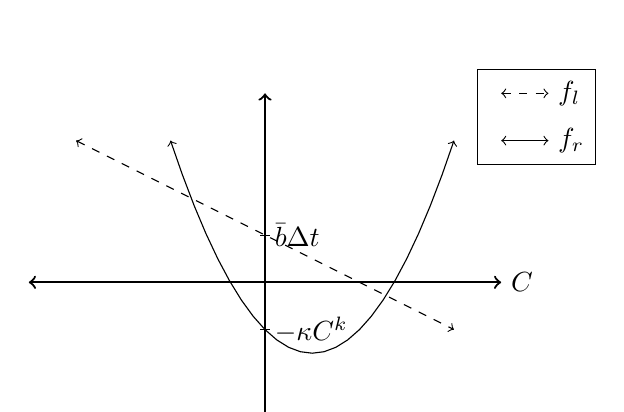
\begin{tikzpicture}[scale=0.6]
    \draw[<->, thick] (-5, 0) -- (5, 0);
    \draw[<->, thick] (0, -3) -- (0, 4); 
    \node[right] at (5, 0) {$C$};
    \node[above] at (0, 4) {};

    \draw[<->, domain=-2:4] plot (\x, {0.5*\x*\x - \x - 1});
    \draw (-0.1, -1) -- (0.1, -1);
    \node[right] at (0, -1) {$-\kappa C^{k}$};

    \draw[<->, dashed, domain=-4:4] plot (\x, {-0.5*\x+1});
    \draw (-0.1, 1) -- (0.1, 1); 
    \node[right] at (0, 1) {$\bar{b} \Delta t$};

    \draw (7, 2.5) -- (4.5, 2.5) -- (4.5, 4.5) -- (7, 4.5) -- (7, 2.5);
    \draw[<->, dashed] (5, 4) -- (6, 4);
    \node[right] at (6, 4) {$f_l$};
    \draw[<->] (5, 3) -- (6, 3);
    \node[right] at (6, 3) {$f_r$};

  \end{tikzpicture}
  &
  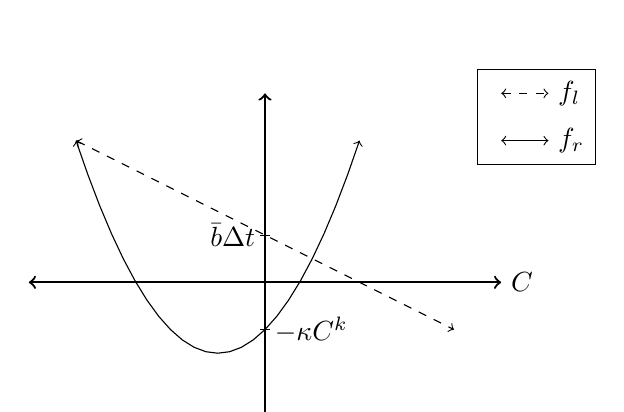
\begin{tikzpicture}[scale=0.6]
    \draw[<->, thick] (-5, 0) -- (5, 0);
    \draw[<->, thick] (0, -3) -- (0, 4); 
    \node[right] at (5, 0) {$C$};
    \node[above] at (0, 4) {};

    \draw[<->, domain=-4:2] plot (\x, {0.5*\x*\x + \x - 1});
    \draw (-0.1, -1) -- (0.1, -1);
    \node[right] at (0, -1) {$-\kappa C^{k}$};

    \draw[<->, dashed, domain=-4:4] plot (\x, {-0.5*\x+1});
    \draw (-0.1, 1) -- (0.1, 1); 
    \node[left] at (0, 1) {$\bar{b} \Delta t$};

    \draw (7, 2.5) -- (4.5, 2.5) -- (4.5, 4.5) -- (7, 4.5) -- (7, 2.5);
    \draw[<->, dashed] (5, 4) -- (6, 4);
    \node[right] at (6, 4) {$f_l$};
    \draw[<->] (5, 3) -- (6, 3);
    \node[right] at (6, 3) {$f_r$};
  \end{tikzpicture}
  \\
  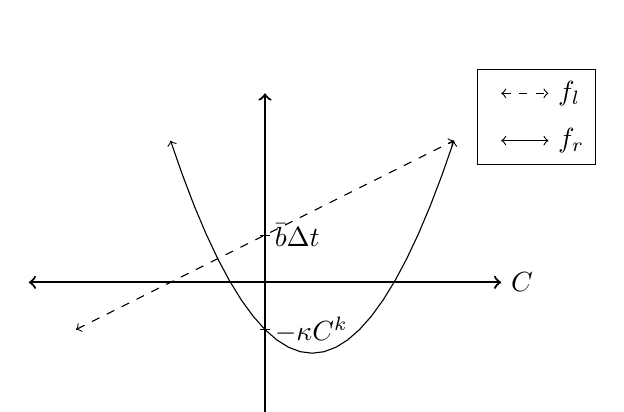
\begin{tikzpicture}[scale=0.6]
    \draw[<->, thick] (-5, 0) -- (5, 0);
    \draw[<->, thick] (0, -3) -- (0, 4); 
    \node[right] at (5, 0) {$C$};
    \node[above] at (0, 4) {};

    \draw[<->, domain=-2:4] plot (\x, {0.5*\x*\x - \x - 1});
    \draw (-0.1, -1) -- (0.1, -1);
    \node[right] at (0, -1) {$-\kappa C^{k}$};

    \draw[<->, dashed, domain=-4:4] plot (\x, {0.5*\x+1});
    \draw (-0.1, 1) -- (0.1, 1); 
    \node[right] at (0, 1) {$\bar{b} \Delta t$};

    \draw (7, 2.5) -- (4.5, 2.5) -- (4.5, 4.5) -- (7, 4.5) -- (7, 2.5);
    \draw[<->, dashed] (5, 4) -- (6, 4);
    \node[right] at (6, 4) {$f_l$};
    \draw[<->] (5, 3) -- (6, 3);
    \node[right] at (6, 3) {$f_r$};
  \end{tikzpicture}
  & 
  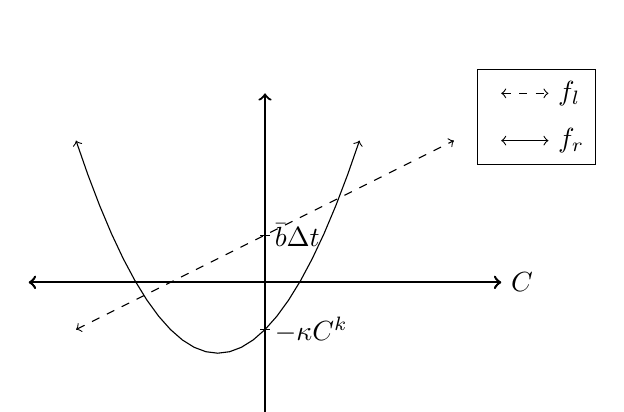
\begin{tikzpicture}[scale=0.6]
    \draw[<->, thick] (-5, 0) -- (5, 0);
    \draw[<->, thick] (-5, 0) -- (5, 0);
    \draw[<->, thick] (0, -3) -- (0, 4); 
    \node[right] at (5, 0) {$C$};
    \node[above] at (0, 4) {};

    \draw[<->, domain=-4:2] plot (\x, {0.5*\x*\x + \x - 1});
    \draw (-0.1, -1) -- (0.1, -1);
    \node[right] at (0, -1) {$-\kappa C^{k}$};

    \draw[<->, dashed, domain=-4:4] plot (\x, {0.5*\x+1});
    \draw (-0.1, 1) -- (0.1, 1); 
    \node[right] at (0, 1) {$\bar{b} \Delta t$};

    \draw (7, 2.5) -- (4.5, 2.5) -- (4.5, 4.5) -- (7, 4.5) -- (7, 2.5);
    \draw[<->, dashed] (5, 4) -- (6, 4);
    \node[right] at (6, 4) {$f_l$};
    \draw[<->] (5, 3) -- (6, 3);
    \node[right] at (6, 3) {$f_r$};
  \end{tikzpicture}
\end{tabular}
\caption{Graph of $f_l = \left( C \right)^2 + \left(\kappa - C^{k}\right)C - \kappa C^{k}$ and $f_r =  \left(\bar{b} - \bar{a} C \right) \Delta t$ for all four possible cases.
  Notice that because $-\kappa C^{k} < 0$ and $\bar{b} \Delta t > 0$ for all realistic parameter values the two functions will always intersect in the positive $C$ region.
  The top left graph is for $\bar{a} > 0$ and $\kappa - C^k < 0$.
  The top right graph is for $\bar{a} > 0$ and $\kappa - C^k > 0$.
  The bottom left graph is for $\bar{a} < 0$ and $\kappa - C^k < 0$.
  The bottom right graph is for $\bar{a} < 0$ and $\kappa - C^k > 0$.
}
\label{fig:proof_pos_sol}
\end{figure}
  
To determine which branch of (\ref{eq:Cquad}) to use, we look at the function logically.
If we know that one positive solution will always exist then the only branch for that to occur is the positive branch.
This is because the square root term, $\sqrt{b^2 -4c}$ will never be negative.
The addition of two negative numbers cannot result in a positive solution therefore the positive branch must be used for the positive solution that we desire.

Now that computable solutions for $M$ and $C$ at a single time step have been found, an algorithm to solve for the next time step can be established.
Algorithm \ref{alg:iterateCM} shows the organization of solving (\ref{equ:C_fixed_point} - \ref{equ:M_fixed_point}). 
\begin{algorithm}
  \KwData{$M^{k}$, $C^{k}$ are vectors with values from the previous time step and $p = 0$. }
  \Begin
  {
    Let $M^{(p=0)} = M^{k}$ and $C^{(p=0)} = C^{k}$\;
    \While{Convergence is not achieved } 
    {
        Solve $A^{(p)} M^{(p+1)} = \frac{1}{\Delta t}M^{(p)}$\;
        Solve $C^{(p+1)} = \frac{1}{2} \left( b \pm \sqrt{b^2 - 4c} \right)$\;
        Check convergence, (\ref{equ:iteration_convergence}\; 
        Let $p = p + 1 $\;
    }
    Let $P := p$\;
    Let $M^{(k+1)} = M^{(P)}$ and $C^{(k+1)} = C^{(P)}$\;
  }
  \caption{Algorithm for the fully-implicit solving of (\ref{equ:model_system}) }
  \label{alg:iterateCM}
\end{algorithm}

Note that Algorithm \ref{alg:iterateCM} actually describes both a fully-implicit and a semi-implicit method for solving (\ref{equ:model_system}). 
Recall that the final number of iterations is recorded as $P$, if $P = 1$ then only a single iteration of the algorithm is applied, which correlates to the behaviour of the semi-implicit method.
This can be produced by selecting a sufficiently large enough tolerance so that the convergence check, (\ref{equ:iteration_convergence}), is always resolved after the first iteration.
The resulting semi-implicit method is effectively the method described in \cite{sirca2012computational}, which was first introduced in \cite{eberl2007finite}.




\section{Implementation}

The implementation of Algorithm \ref{alg:iterateCM} was done with Fortran. The matrix system was converted into a 1D array by use of a bijective mapping defined as:
\begin{equation}
\begin{aligned}
  \pi : \{ 0, \ldots, n\} \times \{0, \ldots, m\} &\to \{1, \ldots, (n+1)(m+1) \}
  (i,j) & \to \pi(i,j)
\end{aligned}
\end{equation}

% I have a figure for this?!?!?!?

The matrix was stored in diagonal format since $A$ is a five-diagonal matrix.

All the computations were run on a custom built workstation with an Intel Xeon CPU E5-2650 (1.2 GHz, 20MB cache size) and 32 GB RAM under Red Hat Enterprise Linux Server release 6.5 (Santiago). 
Running the computations with OpenMP, took advantage of 6 out of the 16 processors of the Intel Xeon CPU, each with 2 threads.
The GNU Fortran compiler, version 4.4.7, was used for all computations; the compiler arguments were
\begin{verbatim} -03 -fdefault-real-8 -fopenmp \end{verbatim}


%\chapter{Simulation}
%\section{Simulation Description}

This will be a short section describing what the region/xgridsize/parameters etc. will be for the following simulations.
The main idea here is so that the results can be appropiatly reproduced. 
Also include a section on the machine run (so this will be reckoning2 I think....)

This will list, in depth, the programs that I use, ie. R, python, Fortran, BASH, and what versions of each.
Should probably also list hat each parameters that isn't method specific ($\alpha, \beta ,\gamma, \delta, \nu, \mu, \kappa$), so mainly the region, gridsize, and t stuff.

\subsection{$CO_2$ Production}

I think describing what the CO2 production equation stuff is here would be best. The idea would be to source the origins of this idea (Alex paper?) and then have the equations and calcuations to figuring it out listed here. Finishing this off with the actual third equation:
\begin{equation}
 \mathcal{P}(t) = \int^t_0 \mathcal{R}(s) dt
\end{equation}
\begin{equation}
 \mathcal{R}(t) = \int_\Omega p_t dx = \int_\Omega G(C) M dx
\end{equation}

A few things that would needed to be added would be to firstly, reverse the order of the introduction of that. Ie. $p_t = G(C) M$ first, then $\mathcal{R}(t) = \ldots$, lastly $\mathcal{P}(t) =\ldots$. Also should have a quick blerb that mentions that $\mathcal{R}(t)$ is the rate of CO2 being produced at the point in time and $\mathcal{P}(t)$ is the cumulative amount of CO2 produced.

%\section{Typical Simulation}

THe main point here is to show the results, visually, of a typical simulation.
This means there will be a number of points to discuss here:
\begin{itemize}
  \item Describe the initial conditions and region
  \item Give a verbal description of what the simulation will be.
  \item Show the parameter values
  \item Show the results.
\end{itemize}

%
%
%This will be a short section describing what the region/xgridsize/parameters etc. will be for the following simulations.
%The main idea here is so that the results can be appropiatly reproduced. 
%Also include a section on the machine run (so this will be reckoning2 I think....)
%
%This will list, in depth, the programs that I use, ie. R, python, Fortran, BASH, and what versions of each.
%Should probably also list hat each parameters that isn't method specific ($\alpha, \beta ,\gamma, \delta, \nu, \mu, \kappa$), so mainly the region, gridsize, and t stuff.

%!% Actually, describe CO2 prod after typical simulation
%
%\subsection{$CO_2$ Production}
%
%I think describing what the CO2 production equation stuff is here would be best. The idea would be to source the origins of this idea (Alex paper?) and then have the equations and calcuations to figuring it out listed here. Finishing this off with the actual third equation:
%\begin{equation}
% \mathcal{P}(t) = \int^t_0 \mathcal{R}(s) dt
%\end{equation}
%\begin{equation}
% \mathcal{R}(t) = \int_\Omega p_t dx = \int_\Omega G(C) M dx
%\end{equation}
%
%A few things that would needed to be added would be to firstly, reverse the order of the introduction of that. Ie. $p_t = G(C) M$ first, then $\mathcal{R}(t) = \ldots$, lastly $\mathcal{P}(t) =\ldots$. Also should have a quick blerb that mentions that $\mathcal{R}(t)$ is the rate of CO2 being produced at the point in time and $\mathcal{P}(t)$ is the cumulative amount of CO2 produced.
%The system
%\begin{align}
%    M_t &= \nabla_x \left( D(M) \nabla_x M \right) + f(C) M \\
%    C_t &= - g(C) M 
%\end{align}
%where
%\begin{align}
%    D(M) &= \delta \frac{M^\alpha}{(1 - M)^\beta} \\
%    f(C) &= g(C) - \nu  \\
%    g(C) &= \frac{\gamma C}{\kappa +C}
%\end{align}
%is solved on a rectangular region with length $L$ and width $\lambda L$ with the following parameter values,
%\begin{equation}
%\begin{aligned}
%    \alpha &= 4 \\
%    \beta &= 4 \\
%    \nu &= 0.1 \\      
%\end{aligned}
%\qquad
%\begin{aligned}
%    \delta &= 10^{-8} \\
%    \kappa &= 0.01 \\
%    \gamma &= 0.81 \\
%\end{aligned}
%\end{equation}
%and with initial conditions of $C = 1$ everywhere and $i$ random innoculation points centered at $(x_i, y_i)$ defined by, 
%\begin{equation}
%  M(x,y) = \max \left\{ -\frac{h}{d^2} \left((x-x_i)^2 + (y-y_i)^2\right) + h, \quad 0 \right\}
%\end{equation}  
%where $h = 0.1/i, d=\frac{5}{128}$ , representing the height and depth of the inoculation site.
%
%Using simulation code version $139e63e$ a typical simultation with $i = 4$ random innoculation points was run. The following results were found using a finite difference method to solve $M$ and trapizedral rule to solve $C$ with $\Delta x = \frac{1}{512}$ and $\Delta t = 10^-2$.
%
%\begin{figure}[h!tb]
%\begin{center}
%  \begin{tabular}{c c}
%%      \includegraphics[scale=0.15]{3d_sim_t0.png} &
%%      \includegraphics[scale=0.15]{3d_sim_t8.png} \\
%      (a) & (b) \\
%%      \includegraphics[scale=0.15]{3d_sim_t16.png} &
%%      \includegraphics[scale=0.15]{3d_sim_t24.png} \\
%      (c) & (d) \\
%%      \includegraphics[scale=0.15]{3d_sim_t32.png} &
%%      \includegraphics[scale=0.15]{3d_sim_t40.png} \\
%      (e) & (f)
%   \end{tabular}
%  \caption{Solutions of $M$ at (a) t = 0, (b) t =8, (c) t = 16, (d) t = 24, (e) t = 32, (f) t = 40. } 
%  \label{fig:solution42}
%\end{center}
%\end{figure}
%
%

%\section{Travelling Wave Analysis}

%%%%%%%%%%%%%%%%%%%%%%%%%%%%%%%%%%%%%%%%%%%%%%%%%%%%%%%%%%%
\subsection{Spatial Simplification}

To simplify the travelling wave analysis we reduce the spatial dimensions to that of a 1D problem.
This can be done if initial conditions that are homogenous with respect to $y$ are chosen.
The purpose of this spatial simplification is that this will speed up the computations considerable.
It will also make visualizations easier as certain figures would become too cluttered in 2D.
What is done here is more of a pseudo-reduction of dimensions.
By reducing the grids from an $n \times m$ grid to an $n \times 4$ grid we have changed the way the problem size scales with finer grids.
The problem is still 2D, just now one dimension has been reduced to only 4 grid points of accuracy instead of $m$ points.
This does not effect the final result since we only apply this change to problems with appropriate initial conditions.
These initial conditions are homogenous in the $y$ direction and thus we do not have any fluctuation between $y$ values for a given $x$ value.

One main benefit of changing the grid from $n \times m$ to $n \times 4$ is that the growth of the problem with respect to the resolution of the grid is reduced dramatically.
This changes the problem from a $O(n^2)$ problem to a $O(n)$.
Using the travelling wave 1D initial conditions, (\ref{equ:basic_init_trav_wave}), one simulation is computed with a $513 \times 513$ grid, seen at Figure \ref{fig:show_dimension_3D}, and another with a $513 \times 4$ grid, seen at Figure \ref{fig:show_dimension_2D}.

\begin{figure}[!htp]
  \centering
  \begin{tabular}{c c}
    \includegraphics[scale=0.7]{show_dimension_3D.eps} &
    \includegraphics[scale=0.7]{show_dimension_3D_side.eps} \\
    (a) & (b) \\
  \end{tabular}
  \caption{Graph of (a) 3D view of $M(t,x,y)$ and $C(t,x,y)$, (b) Side profile view of $M(t,x,y)$ and $C(t,x,y)$ at $t=40$.} 
  \label{fig:show_dimension_3D}
\end{figure}
   
Before any changes to the grid can be made, it must be confirmed that fluctuations are sufficiently small.
To this end, the standard deviation is used as a measure.
The standard deviation is calculated along the $y$-direction for each x value.
This gives a numerical quantity for the measure of dispersal each $y$ value has with another.
Here, we use the sample standard deviation for the sole reason that this single simulation does not represent its own population.
Initially, at $t =0$ the standard deviation is 0 everywhere (DATA NOT SHOWN).
At $t = 40$, Figure \ref{fig:show_dimension_stddev} show the standard of each $y$ value.
After many time steps have passed the amount of spread is always less then $10^{-14}$, which is an acceptable degree of consistency.
Note that the main inconsistency is at the wave front, around $x = 5.75$, which is mainly because of the sharp change in values.

\begin{figure}[!htp]
  \centering
  \includegraphics{show_dimension_stddev.eps}
  \caption{The standard deviation at the same time as the above graphs}
  \label{fig:show_dimension_stddev}
\end{figure}

When simulations are computed with a $n \times 4$ grid, they are still 2D problems.
With regards to visualizations, side profiles could be used on these solutions to present pseudo-1D visualization but this is not ideal.
To visualize the solutions in true 1D the we use $\bar{M}$ and $\bar{C}$ as averaged values of the solutions along the y-axis.
This is computed after the solution has been determined and is independent of the actual computations for M and C.
So by taking the average of the points along the $y$-axis we can get a 2D plot as seen in Figure \ref{fig:show_dimension_2D}. 
 
\begin{figure}[!htp]
  \centering
    \includegraphics{show_dimension_2D.eps}
    \caption{Graph of M(2,y) and C(2,y), now reduced to a 2D plot.}
    \label{fig:show_dimension_2D}
\end{figure}

This means that the system (\ref{equ:model_system}) - (\ref{equ:model_functions}) can be reduced to a $1D$ problem. 
With initial conditions that are homogenous with respect to y, we can greatly reduce the accuracy in the one axis.
Once the y-axis reduced, we can also ignore it for visualizations, only using the x-z axis and plotting the values of $\bar{M}$ and $\bar{C}$.


%%%%%%%%%%%%%%%%%%%%%%%%%%%%%%%%%%%%%%%%%%%%%%%%%%%%%%%
\subsection{Travelling Wave Solution}


%!% section 1.2.2 i think before you discuss travelling waves, you should define what they are. Just take it from my old paper
Classical travelling wave solutions are solutions that propagate with an \textit{a priori} unknown constant speed without any change in shape.
This means that the solutions can be defined as 
\begin{equation}
  M(t,\tilde{x}) = M(\tilde{x} - ct)
\end{equation}
Figure \ref{fig:trav_wave_solution} shows the time evolution of the single time snapshot from Figure \ref{fig:show_dimension_2D}.
Given the above definition and by looking at the consistent appearance of the solution, it suggests that it is a travelling wave.
It is clear here that the shape of the solution is consistent enough to suggest the existence of a travelling wave solution.

\begin{figure}[!htp]
  \centering
  \begin{tabular}{c c}
      \includegraphics[scale=0.55]{trav_wave_solution_t0.eps} &
      \includegraphics[scale=0.55]{trav_wave_solution_t20.eps} \\
      (a) & (b) \\
      \includegraphics[scale=0.55]{trav_wave_solution_t40.eps} & 
      \includegraphics[scale=0.55]{trav_wave_solution_t60.eps} \\
      (c) & (d) 
  \end{tabular}
  \caption{Solutions of $M(x,t)$ and $C(x,t)$ at (a) t = 0, (b) t = 20, (c) = 40, (d) = 60. 
    This was run on a $513 \times 4$ grid.}
  \label{fig:trav_wave_solution}
\end{figure}

The existence of a travelling wave solution for this simulation can be confirmed if the solution $M(x,t)$ can be shown as $M(x-ct)$, where $c$ is the \textit{a priori} unknown wave speed.
Visually, multiple time steps horizontally translated onto each other would show this.
If the horizontal translations are all multiples of the same number then we have shown that a constant speed exists.
If the shape of all the time steps match then a constant shape then strong evidence that a constant shape exists would be shown.
We can numerically approximate the value for $c$ by looking at how fast the peak of the wave travels.
The location of the wave peak is the x coordinate that corresponds to the largest $M$ value.
Recall that we are dealing with a pseudo-1D problem, so there does not need to be any consideration for an $(x,y)$ coordinate.
For this case, we used the GNUPLOT software to fit a linear model, $f(x) = mx + b$, to the last half of the wave peaks path, seen in Figure \ref{fig:trav_waveSpeed}.
The last half of the values were used instead of the whole set of values because only for the former do we have a fully formed travelling wave.
The value of $m$ in $f(x)$ is the approximation for the wave speed, $c$. 

\begin{figure}[!htp]
  \centering
    \includegraphics[scale=0.85]{trav_wavespeed.eps}
    %!% At some point, try to get a line in the graphic that show the region that was used for the fitting.
    \caption{The $x$ location of the wave peak as a function of $t$.
      The red line is the wave peak location extracted from the simulation results.
      The green line is the function $f(x) = cx + b$ with c as the wave speed, found by fitting the model to the second half of x values.
      The simulation results used here are from the solution shown in the previous Figure.
    }
    \label{fig:trav_waveSpeed} 
\end{figure}

With an approximation for $c$, the solutions of Figure \ref{fig:trav_wave_solution} can be represented as $M(x - c (t_0 - t_{n}))$, where $t_0 = 60$ is a reference point for the other time steps.
The values of $t_{n}$ are the times for the other solutions.
By translating along the $x$-axis multiple solution profiles can be superimposed, as seen in Figure \ref{fig:trav_wave_translation}.
The shape of each time step is very similar throughout, only differing slightly at the tail.

\begin{figure}[!htp]
  \centering
    \includegraphics[scale=0.85]{trav_wave_translation.eps}
    \caption{Solutions of $M$ that are represented as $M(x -ct)$ \textit{a priori}.
      The multiple time steps are translated on top of another by horizontal movements of $c (t_0 - t_n)$ for each time step.
      }
    \label{fig:trav_wave_translation}
\end{figure}

Based on the above evidence, we can say that a travelling wave solution has been shown to exist for a single initial condition and particular set of parameters.
This leads to two logical extensions, looking at the stability of the travelling wave solution based on initial condition and investigating the effect the parameters have on the travelling wave solution.

%%%%%%%%%%%%%%%%%%%%%%%%%%%%%%%%%%%%%%%%%%%%%%%%%%%%%%%%%%%
\subsection{Travelling Wave Stability}

%!% section 1.2.3:  it seems that you are here interested in whether you obtain a 1D travelling wave, i.e. you measure whether your solution deviates from a 1D solution. I am not certain that this is the relevant question. I think the question is whether in a full 2D case you get a travelling wave (which does not need to be a 1D wave but can be a fully 2D solution). Your figure \ref{trav_wavefront} seems to suggest this. We can talk about this in the exam or next week.

Based on the previous example, there seems to exist a travelling wave solution. %!% for the intial condition given in (\ref{equ:basic_init_trav_wave}).
The next step is looking at how different initial conditions could still result in a travelling wave solution.
For this we specifically look at the stability of the solution, does it attract nearby solution into becoming a travelling wave solution or is it only for specific cases that one results.
This will help confirm that the existence of the travelling wave solution is not depended on the single choice of initial condition.

To test this we take an initial condition that is not inherently one dimensional and see if it approaches to the one dimension property.
The choice of IC is to have multiple random spherical inoculation points along the $y=0$ side of the region.
Specifically, we use $(x_r, y_r)$ to represent the center of each random inoculation point.
Here $x_r \in \mathcal{R}$ and $y_r \in [0, 0.1]$.

The equation used for each random spherical inoculation point is,
\begin{equation}
  M = \frac{-h}{d^2} \left( (x - x_r)^2 + (y - y_r)^2 \right) + h, \quad M \ge  0.
\end{equation}
Random inoculation points add to each other if they overlap.
After all the inoculation points have been generated, every value is divide by the total amount of biomass.
This lets the initial condition become a representation for the distribution of random inoculation points in terms of the total amount generated.
A time evolution of the simulation with the above initial condition can been seen in Figure \ref{fig:trav_stability}.
Here it can be observed that the solution $M$ appears to slowly converge to a 1D problem.
This cannot be fully seen since the wave propagation reaches the end of the region before it can become fully one dimensional.

\begin{figure}[!htp]
  \centering
  \begin{tabular}{c c}
      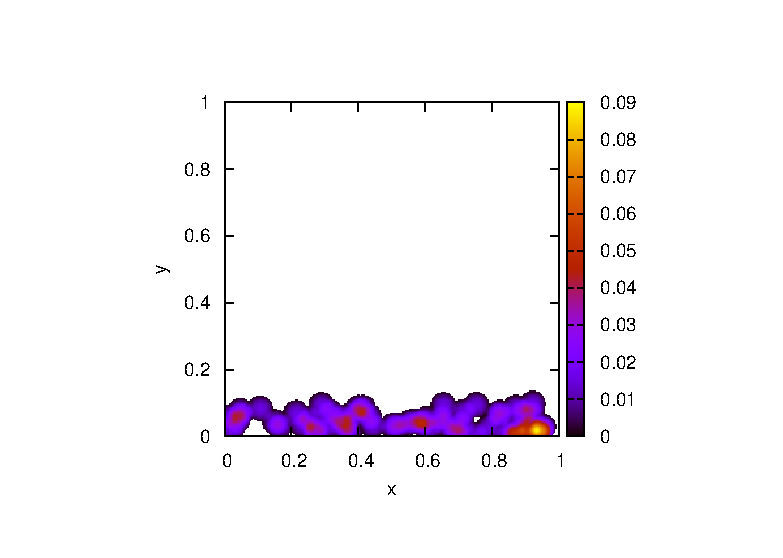
\includegraphics[scale=0.52]{trav_stability_t0.eps} &
      \includegraphics[scale=0.52]{trav_stability_t10.eps} \\
      (a) & (b) \\
      \includegraphics[scale=0.52]{trav_stability_t20.eps} &
      \includegraphics[scale=0.52]{trav_stability_t30.eps} \\
      (c) & (d) 
  \end{tabular}
  \caption{Plots of the simulation with random spherical inoculation points centered in the region $(x,y) \in [0,0] \times [1,0.1]$.
    The solutions are shown at (a) $t = 0$, (b) $t = 10$, (c) $t = 20$, and (d) $t = 30$.
    Each solution is computed on a $513 \times 513$ grid. }
  \label{fig:trav_stability}
\end{figure}

\begin{figure}[!htp]
  \centering
  \includegraphics[scale=0.95]{trav_stability.eps}
  \caption{The standard deviation of the wavefront interface as a function of time.
    The wavefront references the largest $y$ coordinate with $M > 0.001$ for each x coordinate.
    The choice of using $M > 0.001$ is because we want to ignore the small values ($~10^{-100}$) that arise from the diffusion right at the wave front. 
    This simulation is the same as the previous Figure.  }
  \label{fig:trav_stability_stddev}
\end{figure}

We can quantitatively see the behaviour of this convergence by calculating the measure of spread at the wave front.
This can be achieved by calculating the standard deviation of $y$ coordinated for each x coordinate.
By tracking the largest $y$ value with a non-zero $M$ for each x value we can generate a sample data set of the wavefront.
The wavefront is used instead of other points of interest, such as the wave peak, because it is the most consistent of characteristics that can be easily tracked.
As seen in Figure \ref{fig:show_dimension_stddev}, the wave peak had the largest spread among all other values. 

\begin{figure}[!htp]
  \centering
  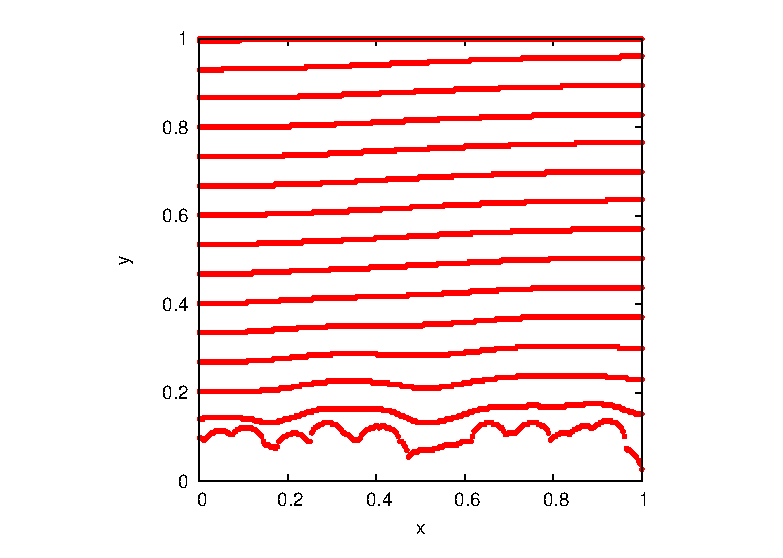
\includegraphics{trav_stability_wavefront.eps}
  \caption{The wavefront shape of multiple time steps.
    Each wavefront has a difference in time by 2, i.e. they are at $t = 4, 6, 8, \ldots, 58, 60$. 
    The simulation results are the same as the previous Figures, using the default parameter values with a grid size $513 \times 513$.
    }
  \label{fig:trav_wavefront}
\end{figure}

Taking the sample standard deviation of this set results in the measure of spread for the wavefront.
The sample standard deviation was used since this one example does not represent the whole population of solutions.
The idea is that, for a solution that converges to one-dimensionality, the $y$ location of the wavefront should be converging to similar values.
This means that the standard deviation would converge to zero.
The standard deviation of the wavefront as a function of time of the simulation ran in Figure \ref{fig:trav_stability} can be seen in Figure \ref{fig:trav_stability_stddev}.
Here is shows that the solution is converging to zero, however not monotonically.
%!% I'm actually not sure what this means.... good news or bad?!

For the numerical computation of the wavefront, the largest $y$ values greater then $0.001$ was used instead of $0$.
The reason is that there are very small values of around $10^{-200}$ that arise due to the diffusion that were not adequate representations of the wavefront.

Another interesting item to investigate is the actual shape of the wavefront.
Figure \ref{fig:trav_wavefront} shows only the wavefront shape for multiple time steps.
The wavefront shape is the same dataset of points used to calculate the standard deviation of the wavefront interface.
Of interest is that the wavefront seems to move at a constant speed, since each wavefront shown is equidistance from the next.


%!% Maybe need to try other types of initial conditions to say this for sure...
% Or maybe just run this same experiment 5 or so times to get a better sample and then just show the stddev of all 5 on a single graph. If they all converge to 0ish then that looks pretty strong.


%%%%%%%%%%%%%%%%%%%%%%%%%%%%%%%%%%%%%%%%%%%%%%%%%%%%%%%%%%%
%!% Here I kinda want to show how the wavespeed dectector script works versus when I use the gnuplot fitting to calculate the wavespeed approximation.
% So here a mention the difference between each calculation and then show the horizontal translation graph for both the script and the fitted wavespeed.
%Show computations for the wave speed

%%%%%%%%%%%%%%%%%%%%%%%%%%%%%%%%%%%%%%%%%%%%%%%%%%%%%%%%%%%
\subsection{Parameter Effect on Wave Speed}

The travelling wave solutions seen before have all existed for a single set of parameters.
Here the four main system parameters, $\delta$, $\kappa$, $\nu$, and $\gamma$ are independent varied and the effect on the travelling wave solutions are observed.
From this we can also see how the wave speed of the travelling wave solution changes as a function of the different model parameters.

\begin{figure}[!htp]
  \centering
  \begin{tabular}{c c}
    \includegraphics[scale=0.55]{parameter_speed_delta.eps} &
    \includegraphics[scale=0.55]{parameter_speed_kappa.eps} \\
    (a) & (b) \\
    \includegraphics[scale=0.55]{parameter_speed_nu.eps} &
    \includegraphics[scale=0.55]{parameter_speed_gama.eps} \\
    (c) & (d) 
  \end{tabular}
  %!% Figure 1.14. the fonts i think are too small; these changes can be made later, not crucial for approving the thesis for defense
  \caption{The value of $c$ as parameter (a) $\delta$, (b) $\kappa$, (c) $\nu$, and (d) $\gamma$ are changed. 
    Note that (a) and (b) have logscales due to the selection of parameter values.
    Each of these were calculated with the same setup as the travelling solution previously done.
    The grid size for each was $513 \times 4$ and a time step of $\Delta t = 0.001$ was used.}
  \label{fig:parameter_speed}
\end{figure}

For this an automated script was created that checks, for each time step, if $M$ is travelling wave solution based on the solution of $M$ from a number of time steps previous.
From this check, a wave speed needs to be approximated based on the distance between the two solutions.
If this approximated wave speed is matched throughout all the x values, then a travelling wave solution is assumed to exist at that time step.
With this script, we can try the same simulation as Figure \ref{fig:trav_wave_solution} with different parameter values.

For each parameter, $\delta$, $\kappa$, $\nu$, $\gamma$, the range of values chosen were arbitrarily.
Figure \ref{fig:parameter_speed} shows the results of the wave speed for each parameter changes.
Mainly it was so that the solution did not propagate too fast and hit the end of the region before developing into a full travelling wave solution.
Generally when the travelling wave does not form it is because the wave front propagates to the end of the region faster then the tail of the travelling wave can decrease to 0.
In the case of $\nu$, any larger values then the selected range resulted in biomass that died faster then it could grow, and thus no travelling wave solution exists.
There did not appear to be any cases were a travelling wave solution could not form.

The behaviour of the wave speed as a result of changing the parameters can be explained by the biological meaning of each parameter.
For $\delta$, the diffusion constant, a large value results in a larger local biomass growth as a result of diffusion.
This speeds up the spreading of the biomass and the propagation of the interface.
For $\kappa$, the half-saturation concentration, this value depicts at what substrate concentration we achieve half-maximum growth for the biomass.
When this value is large, the required amount of substrate for optimal growth speed is increased and thus the overall growth of the biofilm is slowed down.
For $\nu$, the decay and loss rate of biomass, a larger value results in more biomass being ejected from the system and thus the amount of biomass available to grow become smaller and growth propagations are slowed.
For $\gamma$, the biomass yield coefficient, a larger value correlates to a substrate that is quickly consumed which produces less total biomass for growth.
This inhibit the propagation of the biomass interface and lowers the wave speed.
The simulated values recorded in Figure \ref{fig:parameter_speed} agrees with the expected behaviour for each parameter.




%\section{Spatial Effects}

This will be a quick section that goes through:

\begin{itemize}
  \item A quick blerb on what the spatial effects could be and what they can effect. The idea here is that if there are no spatial effects then you can efficently ignore spatial terms and further simplify the model in the future?
  \item Go through the test of showing how two IC that differ spatially (clumped in a corner vs. uniform distribution on one side) talk about the results.
\end{itemize}

%\section{Model Fitting}

This will be the ultimate optional section. The idea here is that the results of $\mathcal{P}(t)$ can possibly be fitted to HErmann's simple ODE that he worked on (with Alex?). If so we can show the reults here. 

%\chapter{Conclusions}
%\section{Lessons Learned}

\begin{itemize}
%  \item What is the main idea of the lesson? From method formulation/validation
%    Where did we learn this from?
%    How does this help things?
  \item From the numerics chapter of the thesis, the validity and usefulness of a newly developed fully-implicit method was investigated.
    By comparing it to the standard semi-implicit method, which it extends, it was determined that a significant accuracy gain results from a single extra iteration of the fully-implicit method.
    Multiple iterations increase this gain since the increase in accuracy is positively correlated to the number of iterations performed.
    However, the computational effort required from the fully-implicit method grows exponentially with lower tolerance.
    The ratio for solution accuracy when weighed against heavier computation times suggests that two iterations of the fully-implicit method is best (one extra from the semi-implicit method).
    This resulted in an extra digit of accuracy at the cost of approximately $150\%$ the computational effort.
  \item From the simulation chapter of the thesis, a number of useful characteristics were observed in the system.
    The existence of travelling wave solutions was strongly suggested from all the evidence gathered.
    The stability of this wave suggests that it always exists, but this cannot be verified due to the analytic complexity of the problem.
    Testing two sets of initial conditions, chosen at opposing extremes of spatial spreading (all biomass in one location versus equally distributed across one boundary), and measuring the $CO_2$ production showed a large difference between the two solutions at a reactor-scale.
    This suggests that two dimensional models are better for accurately mimicking the behaviour of the system.
\end{itemize}

%\section{Future Work}

This will be a quick section.
Mainly have bullet point paragraphs again (like in "lessons learned")
Each bullet paragraph will have:

\begin{itemize}
  \item What could have been changed/improved/explored/avoided?
  \item How could the change be made?
  \item What could this gain?
  \item What possible challenges could this change make?
\end{itemize}

The focus of this section should be for the \textit{non-trivial} points. That is unless it is too difficult to find good points.



\newpage
\pagestyle{References}
\chapter*{References}
\addcontentsline{toc}{chapter}{\hspace{16pt} Complete Bibliography}
\titlespacing{\section}{0pt}{*0}{*0}
\renewcommand{\bibname}{}
\renewcommand\bibsection{}
\titlespacing{\chapter}{0pt}{*0}{*0}
\titlespacing{\section}{0pt}{*0}{*0}
\setlength{\parskip}{0pt}
\setlength{\parsep}{0pt}
\nocite*
\bibliographystyle{plainnat}
\bibliography{ThesisReferences}



\newpage
\pagestyle{fancy}

%%Appendix A Behavioural Plots Simulation Study
%\input{BackMatter/AppendixA}


\newpage
\thispagestyle{custom}
\mbox{}

\end{document}
